\section{Incorporation de connaissance {\it a priori}}\label{incorporation}



\subsection{Notion de crédibilité}\label{credibilite}

Le paradigme bay\'esien critique la notion de {\it confiance statistique classique} : celle-ci n'est pas r\'eellement adapt\'ee \`a une prise de d\'ecision fond\'ee majoritairement sur les observations disponibles,\index{{bay\'esien}@{bay\'esien}} car elle repose sur un comportement d'observations \'equivalentes aux observations r\'eelles, mais r\'ep\'et\'ees \`a l'infini en fonction du mod\`ele choisi. Les arguments permettant de construire ces zones de confiance reposent en effet sur le { comportement en loi} des estimateurs $\hat\theta_n$ (cf. $\S$ \ref{conv.modeles}), qui est en g\'en\'eral connu { asymptotiquement} \index{{asymptotisme}@{asymptotisme}} (soit quand $n\to\infty$). C'est le cas des estimateurs utilis\'es pr\'ec\'edemment pour les mod\`eles de statistique extr\^eme. Or, la seule information dont on dispose sans hypoth\`ese de mod\`ele est l'\'echantillon ${\bf x_n}$, et la taille $n$ de ces donn\'ees peut ne pas \^etre assez grande pour s'assurer d'\^etre ``proche" de l'asymptotisme. \\

\`A cette notion la th\'eorie bay\'esienne substitue celle de {\it cr\'edibilit\'e} \index{{cr\'edibilit\'e bay\'esienne}@{cr\'edibilit\'e bay\'esienne}} : {\bf conditionnellement aux donn\'ees observ\'ees}, une zone de cr\'edibilit\'e estim\'ee contient $\theta$ avec une certaine probabilit\'e. \\

Le conditionnement de $\theta$ aux observations implique alors que $\theta$ est consid\'er\'e non plus comme un vecteur de param\`etres fixes et inconnus, mais comme une variable latente al\'eatoire dont la loi est not\'ee g\'en\'eriquement $\Pi$ (et sa densit\'e $\pi$). L'existence d'une mesure de probabilit\'e sur $\theta$ est attest\'ee par le th\'eor\`eme de repr\'esentation de De Finetti \index{{de Finetti}@{de Finetti}} et ses versions \'etendues  \cite{ONeill2011} lorsque les observations sont simplement consid\'er\'ees comme {\it \'echangeables} (et donc potentiellement d\'ependantes) et non plus {\it iid}. Le cadre bay\'esien englobe donc le cadre classique. %Pour les  mod\`eles extr\^emes, les param\`etres $\theta$ prennent des valeurs dans un domaine $\Theta$ continu\footnote{$\pi$ est donc domin\'ee par la mesure de Lebesgue sur $\Theta$, cf. $\S$ \ref{unidim.chap1}}.  
L'ouvrage \cite{Press2003} (chap. I.5) offre de nombreux d\'etails sur l'existence de $\Pi$ dans un cadre g\'en\'eral. \\

 Le proc\'ed\'e d'inf\'erence \index{{inf\'erence bay\'esienne}@{inf\'erence bay\'esienne}} consiste alors \`a op\'erer une {\it mise \`a jour de la loi $\Pi$} \index{{loi {\it a priori}}@{loi {\it a priori}}} conditionnellement aux observations ${\bf x_n}$, {\it via} la r\`egle de Bayes \cite{Robert2007} : la densit\'e dite {\it a priori} $\pi(\theta)$ est modifi\'ee, par l'ajout d'information issue de la vraisemblance statistique $\ell({\bf x_n}|\theta)$, en une densit\'e {\it a posteriori} $\pi(\theta|{\bf x_n})$ s'\'ecrivant \index{{loi {\it a posteriori}}@{loi {\it a posteriori}}}
\begin{eqnarray}
\pi(\theta|{\bf x_n}) & = & \frac{\pi(\theta) f({\bf x_n}|\theta)}{\int_{\Theta}  \pi(\theta) f({\bf x_n}|\theta) \ d\theta}.\label{bayes}
\end{eqnarray}

Ainsi, l\`a o\`u la statistique classique calcule un estimateur $\hat\theta_n$ (maximisant souvent la vraisemblance $f({\bf x_n}|\theta)$) qui poss\`ede une loi connue asymptotiquement,  la statistique bay\'esienne consid\`ere que la vraie nature de $\theta$ est mieux d\'ecrite par une autre loi statistique qui est d\'efinie \`a taille $n$ fix\'ee, selon l'expression (\ref{bayes}). Des liens profonds existent entre ces deux approches ; en particulier, lorsque $n\to\infty$, les lois respectives de $\hat\theta_n$ et  $\pi(\theta|{\bf x_n})$ deviennent similaires. Ces liens sont pr\'esent\'es en d\'etail dans l'ouvrage de r\'ef\'erence \cite{Robert2007}. \\

La figure \ref{illust-bayes} illustre le positionnement classique de la vraisemblance statistique $f({\bf x_n}|\theta)$, vue comme une fonction de $\theta$, par rapport aux densit\'es $\pi(\theta)$ et $\pi(\theta|{\bf x_n})$ ; la mutualisation des sources d'information sur $\theta$ se traduit logiquement par une distribution {\it a posteriori} plus ``piqu\'ee" -- plus informative donc -- que la loi {\it a priori}\footnote{Except\'e dans les cas o\`u les deux sources d'information sont en d\'esaccord : voir \cite{Evans2006}.}. \\



\begin{figure}[h!]
\centering
\vspace{2cm}
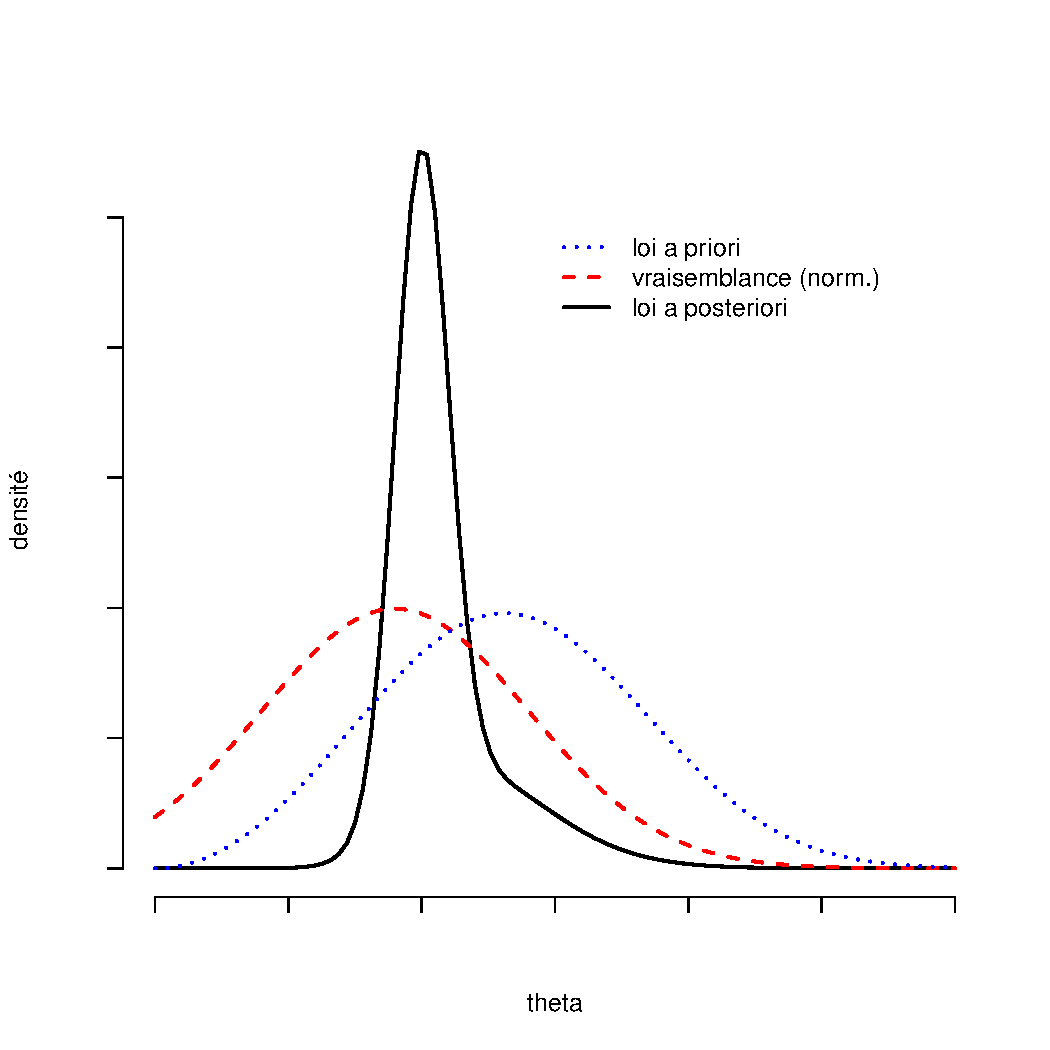
\includegraphics[scale=0.56,natwidth=380,natheight=380]{figures/ex-bayes-1.pdf}
\caption{Illustration par les densit\'es du renforcement de l'information sur $\theta$ \`a partir de la loi {\it a priori} et la vraisemblance des donn\'ees (vue comme fonction de $\theta$ et ici renormalis\'ee). }
\label{illust-bayes}
\end{figure} 




\paragraph*{\bf Nature de la loi {\it a priori}.}
 Qu'exprime la loi {\it a priori} $\pi(\theta)$ ? Un \'etat d'information initial sur les valeurs possibles de $\theta$, ind\'ependant des observations ${\bf x_n}$. Encod\'e sous forme probabiliste, cet \'etat d'information est donc susceptible de permettre l'ajout d'une connaissance r\'eelle et s\'erieuse du ph\'enom\`ene exprim\'ee autrement  qu'au travers d'observations pass\'ees : expertise, pr\'evisions de mod\`eles physiques, etc. Il faut noter que l'information {\it a priori} sur $\theta$ n'est jamais inexistante : en effet, $\theta$ est un choix de param\'etrisation du mod\`ele de vraisemblance, et la structure de ce mod\`ele est connue. En d\'ecoulent des contraintes sur la structure de corr\'elation de $\pi(\theta)$. Nous conseillons au lecteur int\'eress\'e par une pr\'esentation didactique des possibles interpr\'etations de $\pi(\theta)$ l'ouvrage \cite{Parent2007} et l'article \cite{Pasanisi2012}. 
